\documentclass[class=../report, crop=false]{standalone}
\usepackage{graphicx}

\begin{document}

\section{Recommendations}

Our design’s mechanical system is insufficient for the requirements of the competition.
We recommend the adoption of a reliable mechanical design such as that of Team D3 (Figure \ref{fig:d3explode}).

\begin{figure}[H]
	\centering
	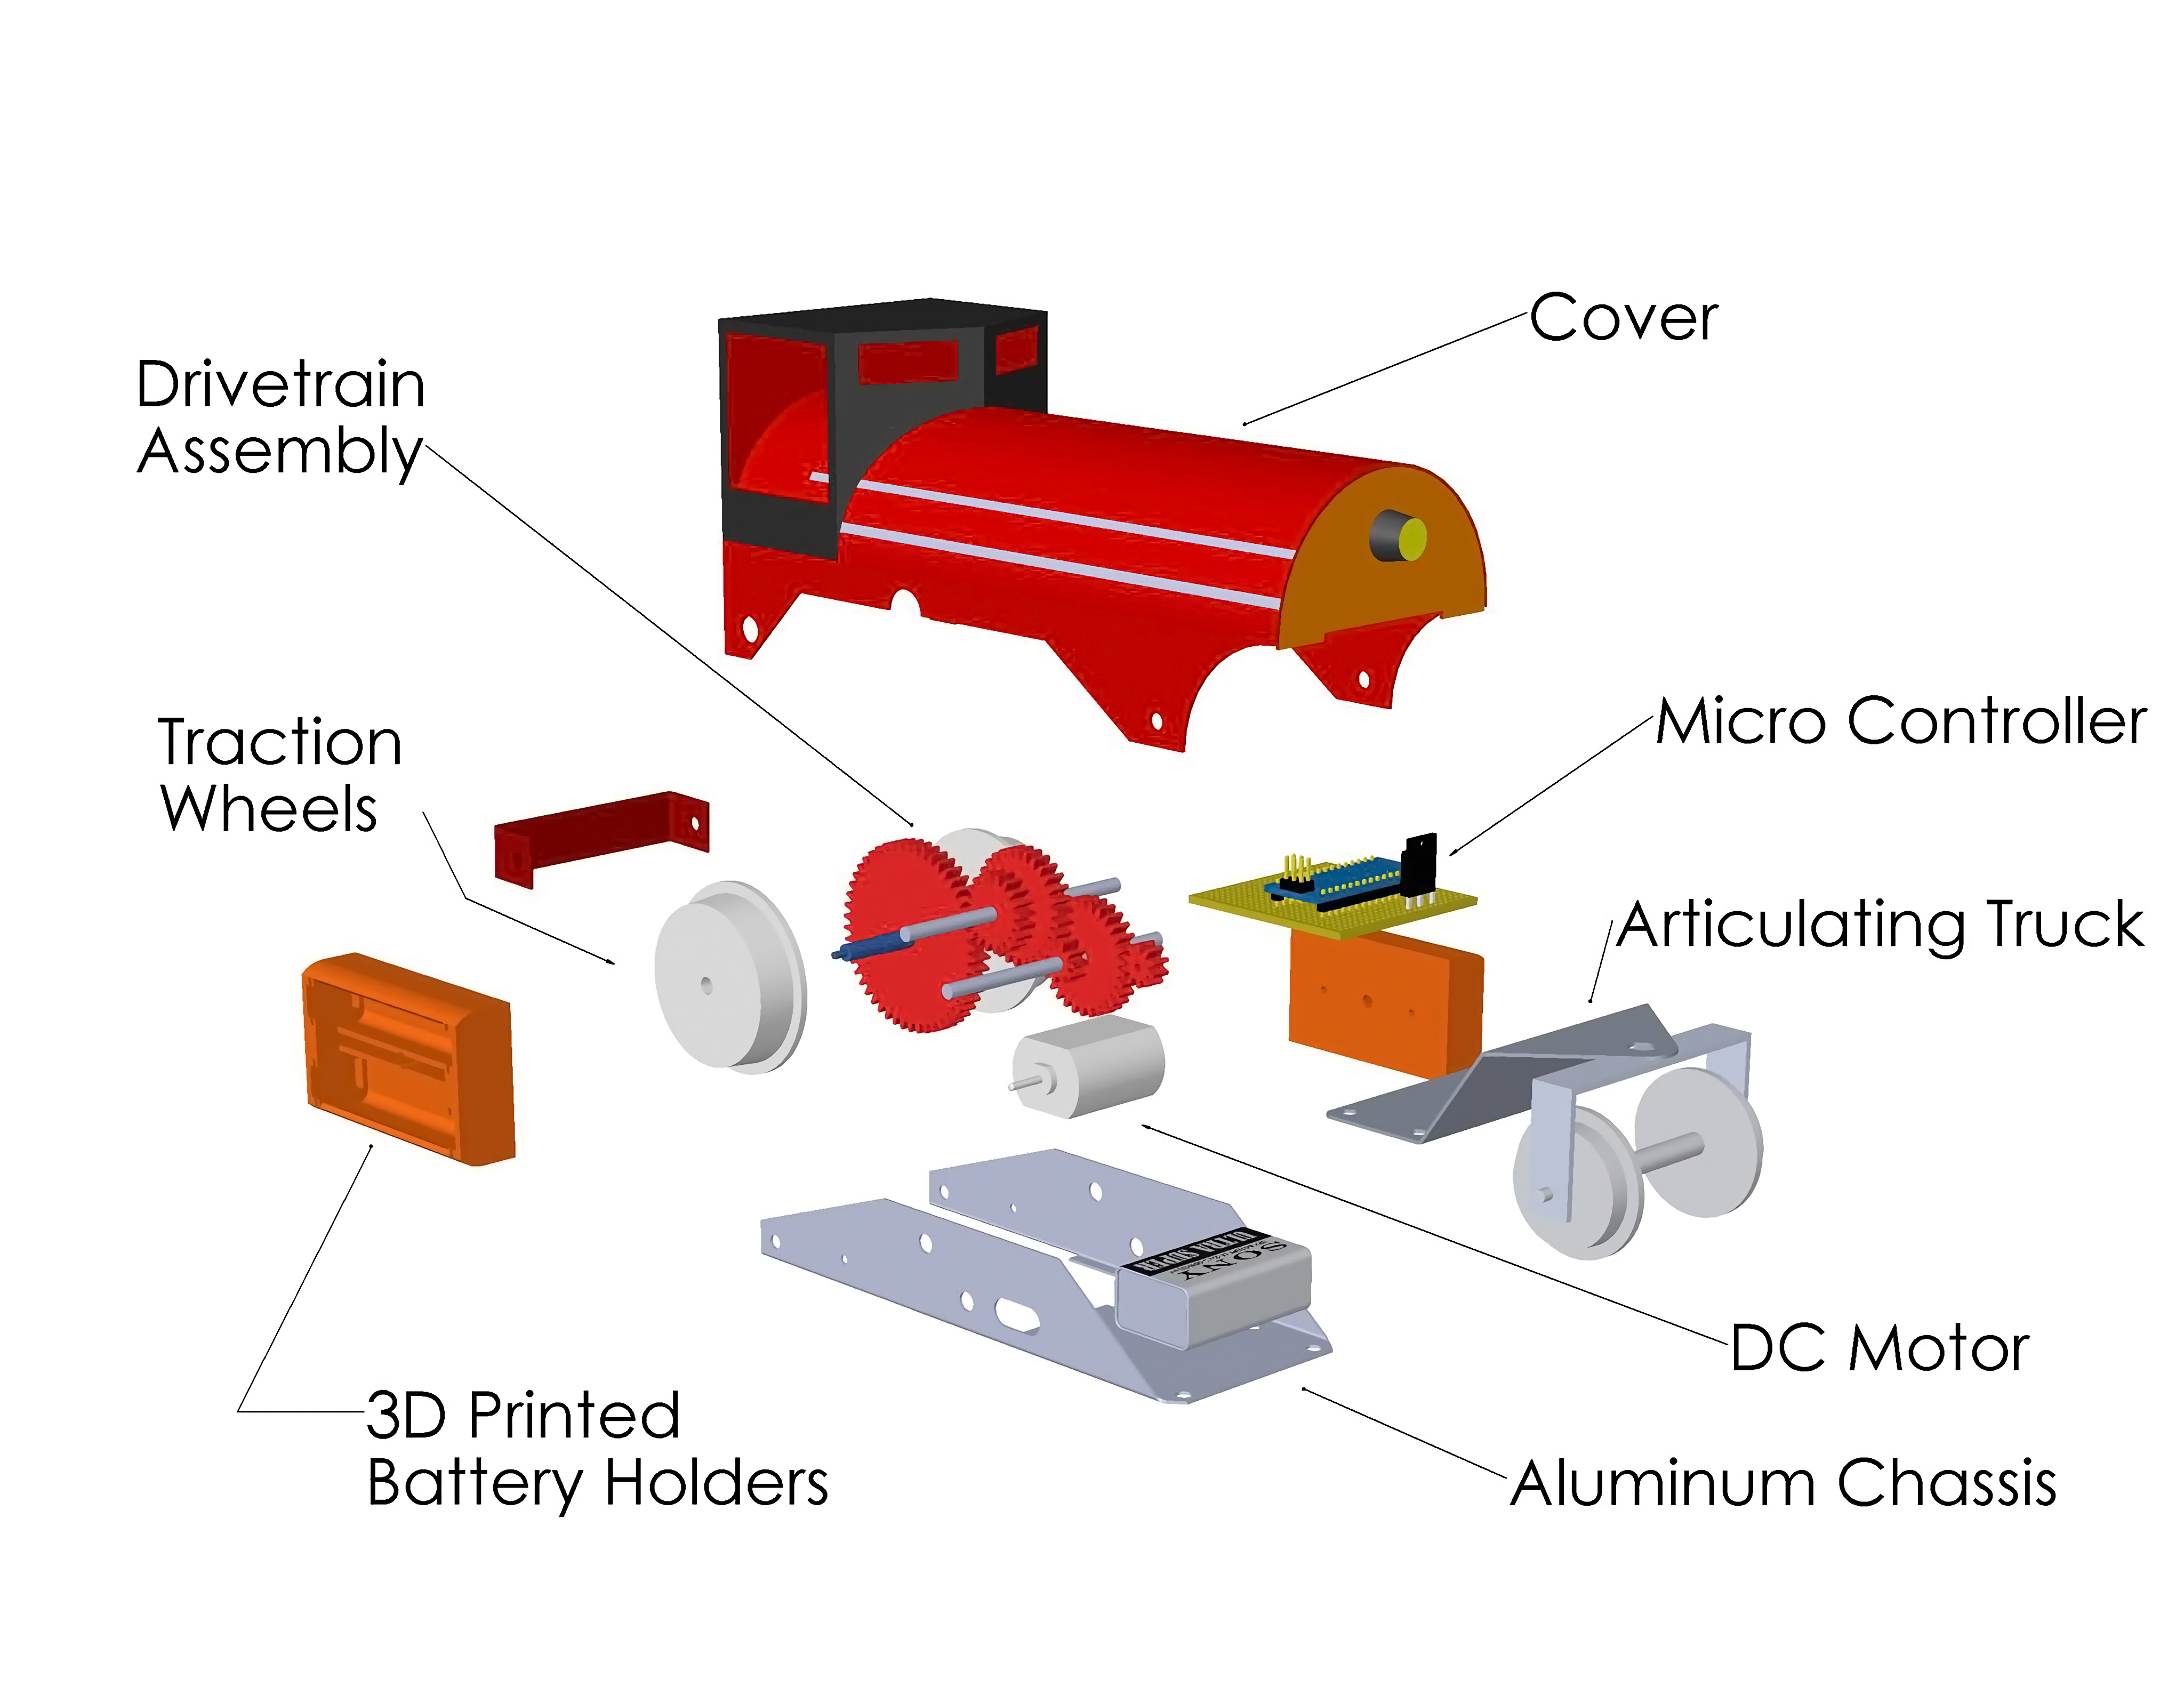
\includegraphics[width=0.8\textwidth]{../res/img/d3explode}
	\caption{Exploded View of Team D3's Design}
	\label{fig:d3explode}
\end{figure}

This design performed well in all rounds of the competition and scored second overall.
We chose not to recommend the first place design (Team D5)  since Team D3’s design is less expensive and is more energy efficient.
The deficiency in performance is minor compared to the lower operational cost of Team D3’s train.

Using Team D3’s design as a model, we recommend the following:
\begin{itemize}
	\item Use a high gear ratio for travelling up inclines and haul cargo
	\item Machine a metal chassis for increased weight and propulsion force
	\item Use a long chassis for placing electrical components close to the track
	\item Include an articulating joint for increased stability
\end{itemize}

Our design has promise if developed further.
However, due to poor implementation and an underestimation of the project’s time constraints, our design is inadequate for competition.
We believe with the improved mechanical system of Team D3’s design, the locomotive would be reliable.
With more available time, we recommend developing an electronic braking system as used in our design.
This electronic braking system offers many advantages over other speed control systems:
\begin{itemize}
	\item Higher speeds on straight sections of track
	\item Lower cost of components
\end{itemize}

With these recommendations, the locomotive would be capable of succeeding in competition; a reliable mechanical system is needed to remove the deficiencies of the current design.

\end{document}
